\section{Background}\label{sc:background}
In this section, we provide a formalization of FMI co-simulation and a brief background on INTO-CPS Maestro 2.

\subsection{FMU definitions}
To describe the formalization of FMUs, we adopt the vocabulary from \cite{gomes_lucio_vangheluwe_2019}. The main definitions of relevance to this paper will be presented, but readers are referred to the original publications for more information. This paper is only concerned with the initialization-phase of a co-simulation, making time of an FMU irrelevant. The formalization from Gomes et al. is extended with new definitions regarding algebraic loops, and convergence of fixed point iteration.
\begin{definition}[FMU]\label{def:fmu}
  An FMU with identifier $c$ is represented by the tuple   
  $$\tuple{\stateset{c}, \inputs{c}, \outputs{c}, \fset{c}, \fget{c}},$$
  where:
  \begin{inparadesc}
    \item $\stateset{c}$ represents the state space;
    \item $\inputs{c}$ and $\outputs{c}$ the set of input and output variables, respectively;
    \item $\fset{c} : \stateset{c} \times \inputs{c} \times \values \to \stateset{c}$ and $\fget{c}: \stateset{c} \times \outputs{c} \to \values$ are functions to set the inputs and get the outputs, respectively (we abstract the set of values that each input/output variable can take as $\values$).
  \end{inparadesc}
\end{definition}

\begin{definition}[Scenario]\label{def:cosim_scenario}
  A scenario is a structure $\tuple{\fmus, \coupling}$ where each identifier $c \in \fmus$ is associated with an FMU, as defined in \cref{def:fmu}, and $\coupling(u)=y$ means that the output $y$ is connected to input $u$.
  Let $\allinputs = \bigcup_{c \in \fmus} \inputs{c}$ and $\alloutputs = \bigcup_{c \in \fmus} \outputs{c}$, then $\coupling : \allinputs \to \alloutputs$.
\end{definition}

The following definitions correspond to the operations that are permitted in the initialization phase of a co-simulation.
\begin{definition}[Output Computation]\label{def:getout}
The $\fget{c}(\dontcare, \outputvar{c})$ represents the calculation of output $\outputvar{c}$ of $c \in \fmus$. Given a co-simulation state, it checks whether all inputs that feed-through to $\outputvar{c}$ are defined.
\end{definition}

\begin{definition}[Input Computation]\label{def:setin}
The $\fset{c}(\dontcare, \inputvar{c}, \inputV)$ represents the setting of input $\inputvar{c}$  of $c \in \fmus$. Given a co-simulation state, it checks whether all outputs connected to $\inputvar{c}$ are defined.
\end{definition}

\begin{definition}[Initialization]\label{def:initialization}
  Given a scenario $\tuple{\fmus, \coupling}$, we define the initialization procedure $\sequence{\initcall_i}_{i \in \setnat}$ as is a finite ordered sequence of FMU function calls that needs to be performed in the initialization of a co-simulation scenario. The ordered sequence is defined as: $\sequence{\functioncall_i}_{i \in \setnat} = \functioncall_0, \functioncall_1, \ldots$ with
  $\functioncall_i \in \initcall_{} = \bigcup_{c \in \fmus} \set{\fset{c},\fget{c}} \cup (\bigcup_{l \in loops} \fixedpoint{l}),$
  and $i$ denoting the order of the function call.
  Fixed point is defined in \cref{def:fixedpoint} and loop in \cref{def:}.
\end{definition}

\begin{definition}[Feed-through]\label{def:feedthrough}
  The input $\inputvar{c} \in \inputs{c}$ feeds through to output $\outputvar{c} \in \outputs{c}$, that is, $(\inputvar{c},\outputvar{c}) \in \feedthrough{c}$, when there exists $v_1, v_2 \in \values$ and $\state{c} \in \stateset{c}$, such that
  $
  \fget{c} (\fset{c}(\state{c}, \inputvar{c}, v_1), \outputvar{c}) \neq \fget{c} (\fset{c}(\state{c}, \inputvar{c}, v_2), \outputvar{c}).
  $
\end{definition}

\claudio{I think the above two definitions should come before the initialization definition, as the later uses the former (I prefer a bottom up approach.). You can also, at the beginning of section 2.1, explain that you're going to ultimately define what the initialization procedure and algebraic loops are, but to do that, you have to define a couple of small things first. This allows the reader to understand why you define these small operations before getting to the bigger definitions.}

\begin{definition}[Interconnected variable]
An interconnected variable v of a co-simulation scenario $\tuple{\fmus, \coupling}$ is defined as $v \in \allinputs \cup \alloutputs$, then $\coupling : \allinputs \to \alloutputs$.
The set all all interconnected variables is denoted: $V = \allinputs \cup \alloutputs$,
\end{definition}

A graph of the dependencies of a co-simulation scenario is established from the interconnected variables by \cref{def:initialization_graph}. The graph is the foundation for the calculation of the initialization procedure and is therefore referred to as the Initialization Graph. The graph construction is similar to the one in \cite{Gomes2019c} except that the later focuses on the co-simulation step, while this work focus on the initialization phase.

\begin{definition}[Initialization Graph]\label{def:initialization_graph}
  Given a co-simulation scenario $\tuple{\fmus, \coupling}$, and a set of feed-through dependencies $\bigcup_{c \in \fmus} \set{\feedthrough{c}}$, we define the Initialization Graph where each node represents a port $\outputvar{c} \in \outputs{c}$ or $\inputvar{c} \in \inputs{c}$ of some fmu $c \in \fmus$. The edges are created according to the following rules:
  \begin{compactenum}
    \item For each $c \in \fmus$ and $\inputvar{c} \in \inputs{c}$, if $\coupling(\inputvar{c}) = \outputvar{d}$, add an edge $\outputvar{d} -> \inputvar{c}$.
    \item For each $c \in \fmus$ and $(\inputvar{c},\outputvar{c}) \in \feedthrough{c}$, add an edge $\inputvar{c} -> \outputvar{c}$.
  \end{compactenum}
\end{definition}

The interconnections of FMU variables can lead to circular dependencies between them, as seen in \cref{fig:fmu_cycle} showing a co-simulation scenario containing an algebraic loop and its Initialization Graph.
\claudio{Simon, can you update the above paragraph to use the co-simulation scenario presernted in the case study section? You can then reuse the space and the reader will already get some familiarity with the case study. Maybe you can even ditch the \cref{fig:fmu_cycle}.}

\begin{figure}
    \centering
    \begin{minipage}{0.55\textwidth}
        \centering
    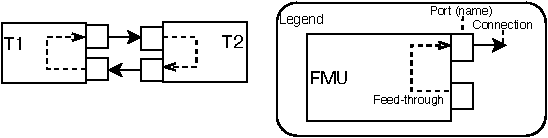
\includegraphics[width=1\textwidth]{images/fmu_cycle.pdf}
    \end{minipage}\hfill
    \begin{minipage}{0.35\textwidth}
        \centering
    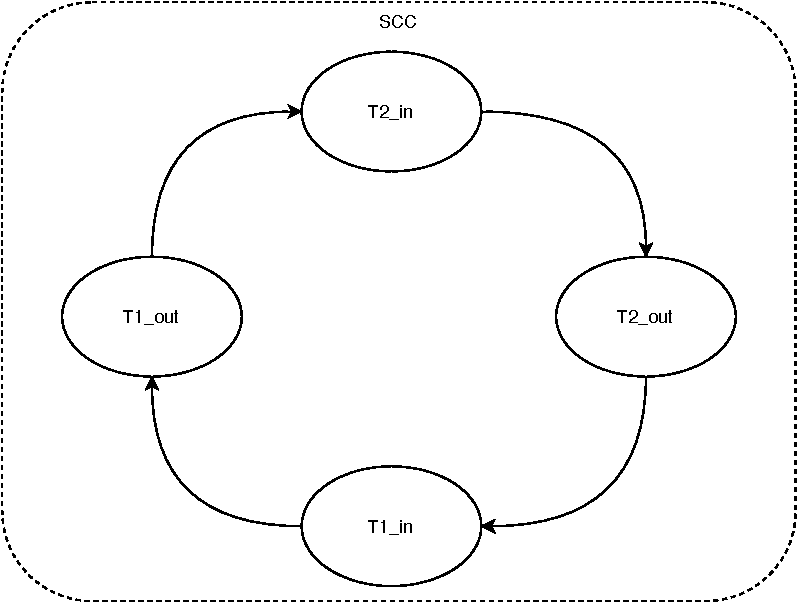
\includegraphics[width=1\textwidth]{images/SCC.pdf}
    \end{minipage}
    \caption{An FMU co-simulation scenario and its Initialization Graph}
    \label{fig:fmu_cycle}
\end{figure}


The following definitions formalizes the concept of an algebraic loop in a co-simulation scenario, and define the problem these algebraic loops are introducing.
The definition of strongly connected components is adapted from the semantics of Causal Block Diagrams (see \cite{Gomes2020} for an overview).

\begin{definition}[Algebraic loops] 
An algebraic loop is defined as a non-trivial strongly connected component of the graph in \cref{def:initialization_graph}.
Formally, a strong connected component satisfies $\set{a,b \in SCC: \mathit{Path}(a,b)}$, where $\mathit{Path}(a,b)$ is true when there's a path (including an empty path) between nodes $a$ and $b$ ($\mathit{Path}(a,a)$ is always true).
An $SCC$ is non trivial when it has more than one node.
%$\LoopVariables = \{v | v \in V : Path(v,v)\}$ \\
%An algebraic loop is defined as the set $\{p_1, p_2 | p_1, p_2 \in \LoopVariables: Path(p_1, p_2) \land Path(p_2, p_1)\}$/
%Path is defined as the transitive closure of the edges of the graph denoted by \cref{def:initialization_graph}.
\end{definition}

Since the edges of the graph represent dependencies between variables, the value of every variable in a non trivial strong component depends on itself.
Let $X$ denote a vector of one or more variables whose value depends on itself. Then the non trivial strong component forms an equation with the form $F(X, U) = X$, where $F$ denotes the relations between the variables in the loop, and $U$ denotes the variables whose values are calculated elsewhere.
This means that algebraic loops need to be handled using fixed point iterations\cite{Gomes2018}. 
% It is a technique to repeatedly perform the steps of a sub-list of the co-simulation step. The number of repetitions the operations should be performed depends on the characteristics of the scenario. The operations should be performed until the system converge. 
An example of applying a fixed point iteration can be seen in \cref{def:fixedpoint} where a system containing an algebraic loop has to be initialized using fixed point iteration.
\claudio{Perhaps later you can ditch \cref{fig:fixedpont} and refer to the case study section, to shorten the text.}
\claudio{You should avoid forcing Latex to position pictures in a particular place. It's bad practice because it causes too much blank space. Also it's a lot of work for you to care about the specific placement of figures.}

\begin{figure}
    \centering
    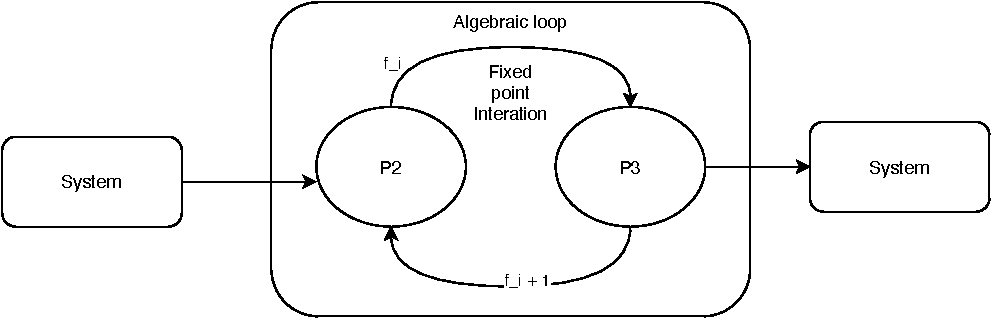
\includegraphics[width=0.8\textwidth]{images/fixedpoint.pdf}
    \caption{Fixed point iteration in a co-simulation scenario}
    \label{fig:fixedpont}
\end{figure}

% The initialization of the system requires the application of fixed point iteration, as defined \cref{def:fixedpoint}.
\begin{definition}[Fixed point iteration of an Initialization procedure]\label{def:fixedpoint}
A fixed point iteration of given loop $l$ consist of the order sequence of functions calls:
$\forall v \in l: \exists op \in \fixedpoint{l} : op = \fget{}(\dontcare, v) \lor op = \fset{}(\dontcare, v, \dontcare)$.
Performing a iteration on a co-simulation state leads to a new state to $\fixedpoint{l}(\state{n}) = \state{n + 1}$
The fixed point iteration is performed in order to find a convergent initialization state as defined in \cref{def:convergence}.
\end{definition}

\claudio{The above defintions is strange. If there's an algebraic loop, you cannot have an initialization procedure. At least not the way it is currently defined. Also I feel that you don't really need to define the fixed point iteration. We just need to reformulate the initialization procedure so that it matches what your plugin should output.}

A fixed point iteration technique is not guaranteed to convergence if the system is unstable. This means that an upper bound of the number of repetitions needs to be established to ensure termination. In case of a non-converging algebraic loop the simulation should be stopped since the result of the co-simulation scenario would not be trustworthy. The criteria of a valid co-simulation scenario is specified in \cref{def:convergence}.

\begin{definition}[Convergence of Fixed point iteration]\label{def:convergence}
A fixed point iteration converges if a finite number of iterations will make the difference of the output value of the same operation between two following iterations within a certain threshold $\epsilon$.\\
Formally, 
$\exists n \in \setnat: |F(X^{n+1}, U) - F(X^{n}, U)| \leq \epsilon$.
\end{definition}

\subsection{INTO-CPS Maestro 2}\todo{We can have some more in this section - Ask Casper if he can do it?}
INTO-CPS Maestro 2\footnote{currently in alpha \url{https://github.com/INTO-CPS-Association/maestro/tree/2.0.0-alpha}}\cite{Thule2019b} is an FMI-based co-simulation framework set to supersede Maestro\cite{Maestro}. The philosophy of the framework is to apply plugins to generate co-simulation specifications expressed in the domain specific language called Maestro Base Language (MaBL). Such specifications are then interpreted and executed, resolving in the execution of a co-simulation.